\documentclass[11pt,border=5pt]{standalone}
\usepackage{fontspec}
\setmainfont{cmunrm.otf}[BoldFont=cmunbx.otf,ItalicFont=cmunti.otf,BoldItalicFont=cmunbi.otf]
\usepackage{amsmath}
\usepackage{unicode-math}
\setmathfont{NewCMMath-Regular.otf}
\usepackage{tikz}
\usetikzlibrary{arrows.meta,patterns,angles,quotes}
\begin{document}
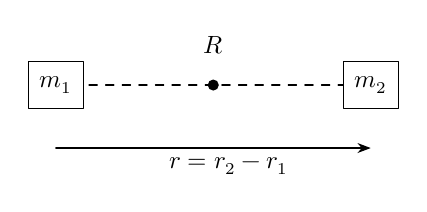
\begin{tikzpicture}[>=Stealth,font=\small,line cap=round,line join=round]
\draw[dashed] (-2,0) -- (2,0);
\draw[fill=white] (-2.35,-0.3) rectangle (-1.65,0.3);
\node at (-2,0) {$m_1$};
\draw[fill=white] (1.65,-0.3) rectangle (2.35,0.3);
\node at (2,0) {$m_2$};
\fill (0,0) circle (2pt);
\node at (0,0.5) {$R$};
\draw[->,thin] (-2,-0.8) -- (2,-0.8) node[pos=0.55,below] {$r=r_2-r_1$};

\end{tikzpicture}
\end{document}
